\chapter{Antipodal double covers of regular graphs}
\label{4classbip}
Let $\Gamma$ be an undirected graph on $v$ vertices. A \emph{projective double}\index{projective double} of $\Gamma$ is an antipodal (spherical) $4$-distance set, say $L = \left\{\ell_1,\dots,\ell_{2v}\right\}$ with inner products $A = \left\{1,\alpha,0,-\alpha,-1\right\}$, such that there exists a mapping $\phi:L\rightarrow V\Gamma$ fulfilling
\begin{enumerate}[label=(\roman*)]
	\item $\phi(\ell_i) = \phi(\ell_j)$ if and only if $\left\vert\left<\ell_i,\ell_j\right>\right\vert = 1$,
	\item $\phi(\ell_i) \sim \phi(\ell_j)$ if and only if $\left\vert\left<\ell_i,\ell_j\right>\right\vert = \alpha$
\end{enumerate}
for $1\leq i,j\leq 2v$. Since the inner products are determined by a single parameter $\alpha$, we will often refer to $L$ as a projective double of $\Gamma$ with inner product $\alpha$. For vertices $v,w\in V\Gamma$, $(ii)$ implies $v\not\sim w$ if and only if $\ell_v\perp\ell_w$ for any $\ell_v\in\phi^{-1}(v)$ and $\ell_w\in\phi^{-1}(w)$. In this Chapter, we investigate such projective doubles and ask which dimensions they exist in for any given graph. Noting a small example, we find that the incidence graphs of such doubles induced by each inner product will, at times, correspond to a 4-class association scheme. We investigate further when this may occur, noting as well the structure which any association scheme arising in this way must take. We finish this chapter by examining 4-class $Q$-bipartite schemes, applying the bounds found in Theorem \ref{schoen-as}. Below are the main results of this chapter.
\begin{restatable*}{prop}{projsrg}\label{projnec}
	A projective double of a simple graph $\Gamma$ induces an association scheme only if $\Gamma$ is strongly regular.
\end{restatable*}
\begin{restatable*}{cor}{cocliquealpha}\label{snegsquare}
	Let $\Gamma$ be a nonempty strongly regular graph with $v$ vertices, valency $k$ and smallest eigenvalue $s$ which contains a Delsarte coclique $C$. Then any projective double in $\mathbb{R}^{\vert C\vert}$ has inner product $\alpha=\sqrt{-s}$. Further, either $\Gamma$ is complete bipartite or $\alpha^{-1}\in \mathbb{Z}$.
\end{restatable*}
\begin{restatable*}{cor}{deliffqbip}\label{deliffqbip}
	Let $\Gamma$ be a strongly regular graph with $v$ vertices, valency $k$, and smallest eigenvalue $s$ which contains a Delsarte coclique. A projective double of $\Gamma$ in dimension $m<v$ induces an association scheme if and only if $m = v\left(1-\frac{k}{s}\right)^{-1}$. Further, the association scheme induced is $Q$-bipartite.
\end{restatable*}

\begin{restatable*}{thm}{fourclasssixzero}\label{thm60}
	Suppose we have a feasible parameter set for a $4$-class association scheme which is $Q$-bipartite but not $Q$-antipodal. Let $k=P_{01}$, $r=P_{21}$, and $s=P_{41}$ where $P$ is the first eigenmatrix using the natural ordering. Then the scheme is realizable only if $s=-n^2$ for some integer $n>1$ and
	\[15n^4(2n^2-3)r^2 + (n^6-45kn^2+76k)n^2r+k(16k+n^6)(n^2-2)\geq 0.\]
\end{restatable*}
\section{Projective doubles of regular graphs}
We begin this section with two propositions concerning projective doubles, first with simple graphs and then with regular graphs.
\begin{prop}\label{dirnaive}
	For any non-empty simple graph $\Gamma$, there exists a projective double in $\mathbb{R}^{m}$ for some $m\leq \vert V\Gamma\vert$ with $\alpha = d^{-1}$ with $d$ the max degree of $\Gamma$.
\end{prop}
\begin{proof}
	Let $\Gamma = \Gamma(V,E)$ be given. Now orient every edge of $\Gamma$ and define $e_i^+,e_i^-\in V$ so that $e_i = (e_i^-,e_i^+)$, thus $e_i$ points from vertex $e_i^-$ to $e_i^+$. Let $M$ be the matrix with rows indexed by vertices and columns indexed by edges such that
	\[\left[M\right]_{ij} =\begin{cases} 1 &\text{ if }v_i = e_j^+\\
	-1 &\text{ if }v_i = e_j^-\\
	0 &\text{ otherwise. }
	\end{cases}\]
	Then we find 
	\[\left[MM^T\right]_{ij} = \begin{cases}
	k_i & \text{ if }i=j,\\
	1 & \text{ if } i\sim j,\\
	0 & \text{ otherwise}
	\end{cases}\]
	where $k_i$ is the degree of vertex $i$. Thus two distinct rows are orthogonal if and only if their corresponding vertices are non-adjacent. However unless $k_i$ is constant independent of $i$ (the graph is regular), the rows do not have the same norm. To solve this, let $d = \max_{i}(k_i)$ (the max degree of $\Gamma$) and define the diagonal matrix $D$ whose $i^\text{th}$ diagonal entry is $\sqrt{d-k_i}$. Then the matrix $N = \left[\begin{array}{c|c}
	M & D
	\end{array}\right]$ has the property that
	\[\left[NN^T\right]_{ij} = \left[MM^T\right]_{ij} + (d-k_i)\delta_{ij} = \begin{cases}
	d & \text{ if }i=j,\\
	1 & \text{ if } i\sim j,\\
	0 & \text{ otherwise.}
	\end{cases}\]
	Thus the rows of $\frac{1}{\sqrt{d}}N$, along with their negatives, result in a projective double of $\Gamma$ with inner product $\frac{1}{d}$. Further the rank of $N$ is no larger than $\max\left\{\vert V\vert, \vert V\vert+\vert E\vert\right\} = \vert V\vert$.
\end{proof}
\begin{cor}\label{regnaive}
	For any regular graph $\Gamma$ with regularity $k>0$, there exists a projective double in $\mathbb{R}^m$ with inner product $\frac{1}{k}$ for some $m\leq T$ where $T$ is the number of edges in any spanning forest.
\end{cor}
\begin{proof}
	We follow the same proof as with Proposition \ref{dirnaive}, however we note that since our graph is regular, the rows of $M$ all have the same norm. Thus the normalized rows (with their negatives) suffice as our projective double. Now, consider any cycle $C$ in $\Gamma$ and assume without loss of generality that $C = \left\{e_1,\dots,e_s\right\}$. Then, replacing a column with its negative if necessary, $\displaystyle{M_{e_s} = \sum_{i=1}^{s-1}M_{e_{i}}}$. We then reorder the columns of $M$ so that the first $T$ edges correspond to the edges of a spanning forest and note that every remaining column induces a linear dependence.
\end{proof}
Proposition \ref{dirnaive} and corollary \ref{regnaive} provide upper bounds on the dimension necessary for a projective double to exist for a given graph. The following observation gives us a lower bound using the independence number of a graph $\alpha\left(\Gamma\right)$.
\begin{prop}\label{cocliquebnd}
	Let $\Gamma$ be a simple graph and $L$ be a projective double of $\Gamma$ in $\mathbb{R}^m$. Then $m\geq \alpha\left(\Gamma\right)$ where $\alpha\left(\Gamma\right)$ is the independence number of $\Gamma$.
\end{prop}
\begin{proof}
	Assume we have a projective double of $\Gamma$ in $\mathbb{R}^m$ with $\phi(\pm\ell_i) = v_i$ for $1\leq i\leq\vert V\vert$. Let $\alpha = \alpha\left(\Gamma\right)$ and without loss of generality let $S = \left\{v_1,\dots,v_\alpha\right\}$ be an independent set. Then $\left\{\ell_1,\dots,\ell_\alpha\right\}$ is an orthonormal set, forcing $m\geq\alpha$.
\end{proof}
We are interested in when we may achieve this lower bound.
\begin{example}\label{doublecoverc4}
Consider the graph $C_4$. This is a regular graph with 3 edges in any spanning tree, thus Corollary \ref{regnaive} tells us there exists a projective double in $\mathbb{R}^3$ with inner product $\frac{1}{2}$. In fact, the columns of $U_1$ serve as one such projective double. 
\[U_1 = \left[\begin{array}{crcccccc}
1 & -1 & \frac{1}{2} & -\frac{1}{2} & 0 & 0 &\frac{1}{2} &-\frac{1}{2}\\
0 & 0 & \frac{\sqrt{3}}{2} & -\frac{\sqrt{3}}{2} & \frac{1}{\sqrt{3}} & -\frac{1}{\sqrt{3}} & -\frac{1}{\sqrt{12}}& \frac{1}{\sqrt{12}}\\
0 & 0 & 0 & 0 & \sqrt{\frac{2}{3}} & -\sqrt{\frac{2}{3}} & \sqrt{\frac{2}{3}} & -\sqrt{\frac{2}{3}} \\			
\end{array}\right]\]
The maximum independent set in this graph has size $2$ and thus Proposition \ref{cocliquebnd} allows for the possibility of a projective double in $\mathbb{R}^2$. While it is not hard to show that we cannot find a projective double in $\mathbb{R}^2$ with inner product $\frac{1}{2}$, we may change the inner product to $\frac{1}{\sqrt{2}}$ and find an example. For instance:
\[U_2 = \left[\begin{array}{crcrcccc}
1 & -1 & 0 & 0 & \frac{\sqrt{2}}{2} & -\frac{\sqrt{2}}{2} & \frac{\sqrt{2}}{2} & -\frac{\sqrt{2}}{2}\\
0 & 0 & 1 & -1 & \frac{\sqrt{2}}{2} & -\frac{\sqrt{2}}{2} & -\frac{\sqrt{2}}{2} & \frac{\sqrt{2}}{2}\\				
\end{array}\right]\]
To see the difference between $U_1$ and $U_2$, consider the graph $\Gamma_\alpha$ on $L$ with $\ell_i\sim\ell_j$ if and only if $\left<\ell_i,\ell_j\right> = \alpha$. Using the columns of $U_1$ as our projective double, we find that $\Gamma_{\frac{1}{2}}$ is given below where $v_i$ represents the $i^\text{th}$ column of $U_1$.
\[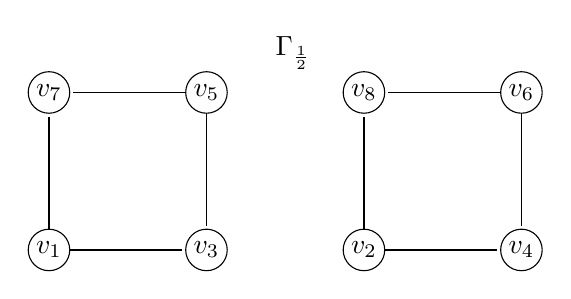
\begin{tikzpicture}[shorten >=1pt,auto,node distance=2cm,
thin,main node/.style = {circle,draw, inner sep = 0pt, minimum size = 15pt}]

\node[main node,fill=white] (1) {$v_1$};
\node[main node,fill=white] [right of = 1](2) {$v_3$};
\node[main node,fill=white] [above of = 1](3) {$v_7$};
\node[main node,fill=white] [above of =2](4) {$v_5$};
\node[main node,fill=white] [right of =2](5) {$v_2$};
\node[main node,fill=white] [right of = 5](6) {$v_4$};
\node[main node,fill=white] [above of = 5](7) {$v_8$};
\node[main node,fill=white] [above of =6](8) {$v_6$};
\node at (3.1,2.5) (9) {$\Gamma_{\frac{1}{2}}$};

\path[-]
(1) edge node {} (2)
edge node {} (3)
(4) edge node {} (3)
edge node {} (2)
(5) edge node {} (6)
edge node {} (7)
(8) edge node {} (7)
edge node {} (6);
\end{tikzpicture}\]
Similarly, if we instead consider $U_2$ as our projective design, $\Gamma_{\frac{\sqrt{2}}{2}}$ is given below.
\[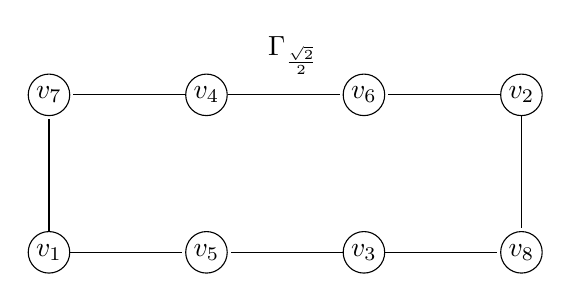
\begin{tikzpicture}[shorten >=1pt,auto,node distance=2cm,
	thin,main node/.style = {circle,draw, inner sep = 0pt, minimum size = 15pt}]
	
	\node[main node,fill=white] (1) {$v_1$};
	\node[main node,fill=white] [right of = 1](2) {$v_5$};
	\node[main node,fill=white] [above of = 1](3) {$v_7$};
	\node[main node,fill=white] [above of =2](4) {$v_4$};
	
	\node[main node,fill=white] [right of =2](5) {$v_3$};
	\node[main node,fill=white] [right of = 5](6) {$v_8$};
	\node[main node,fill=white] [above of = 5](7) {$v_6$};
	\node[main node,fill=white] [above of =6](8) {$v_2$};
	\node at (3.1,2.5) (9) {$\Gamma_{\frac{\sqrt{2}}{2}}$};
	
	\path[-]
	(1) edge node {} (2)
	edge node {} (3)
	(4) edge node {} (3)
	edge node {} (7)
	(5) edge node {} (6)
	edge node {} (2)
	(8) edge node {} (7)
	edge node {} (6);
\end{tikzpicture}\]
Thus $U_1$ and $U_2$ are non-isomorphic as their corresponding graphs are non-isomorphic double covers of $C_4$. Even further, define the five relations $R_0,\dots,R_4$ via the inner products $1$, $\alpha$, $0$, $-\alpha$, and $-1$ respectively so that, for instance, $(x,y)\in R_2$ if and only if the corresponding vectors are orthogonal. These four relations satisfy all the requirements of an association scheme except for possibly the existence of intersection numbers. In the case of the projective double $U_1$, we find that even though $(v_1,v_5)\in R_2$,
\[\left\vert\left\{v_x : (v_x,v_1),(v_5,v_x)\in R_{\alpha}\right\}\right\vert\neq\left\vert\left\{v_x : (v_x,v_1),(v_4,v_x)\in R_{\alpha}\right\}\right\vert.\]
However the projective double $U_2$ has well-defined intersection numbers and we find that the columns of $U_2$, along with the relations $R_0,\dots,R_4$, give the association scheme $C_8$.
\end{example}
As one might expect, there are many graphs for which we cannot find a projective double in the dimension given by the independence number. In other words, Proposition \ref{cocliquebnd} is often not tight. To see an example, consider the following proposition

\begin{prop}
	Let $\Gamma$ be a complete multipartite graph with $w$ parts of size $v$. Let $U$ be the matrix with columns corresponding to a projective double of $\Gamma$ where $\text{rank}\left(U\right) = \alpha\left(\Gamma\right) = v$. Then a subset of the columns of $U$ form a set of $w$ mutually unbiased bases in $\mathbb{R}^v$.\qed
\end{prop}
\begin{proof}
	Follow the same proof as in Proposition \ref{cocliquebnd}, however only consider one line from each antipodal pair. Noting that non orthogonal vectors must have inner product $\pm\alpha$, the result is immediate.
\end{proof}
\begin{cor}\label{nonexist}
	Let $\Gamma = K_{2\times t}$ for $t\neq 0\mod 4$. $\Gamma$ does not have a projective double in $\mathbb{R}^\alpha$ for $\alpha = \alpha\left(\Gamma\right)$.
\end{cor}
\begin{proof}
	If $K_{2\times t}$ had a bipartite double, then it would be a set of two mutually unbiased bases in $\mathbb{R}^t$. This is only possible when $t$ is a multiple of $4$.
\end{proof}

\section{Schemes induced by projective doubles}
Example \ref{doublecoverc4} provides a projective double which naturally gives an association scheme on the vectors. In this section we consider which graphs may produce such an association scheme and some properties of the association scheme which arise. First, let $L$ be a projective double of some graph $\Gamma$ and let $G$ be the Gram matrix of $L$; that is the matrix whose entry in row $i$ and column $j$ is $\left<\ell_i,\ell_j\right>$. We denote by $\left<G\right>_\circ$ the vector space of matrices generated by $G$ using entrywise products. Note that the adjacency matrices of each graph $\Gamma_{\theta}$ for $\theta\in\left\{\pm 1,\pm \alpha,0\right\}$ are all contained in $\left<G\right>_{\circ}$. Thus $\left<G\right>_\circ$ is a Bose-Mesner algebra if and only if it is closed under standard matrix multiplication. If this occurs, we say $L$ induces the corresponding 4-class association scheme. Thus, from example \ref{doublecoverc4}, the association scheme $C_8$ is induced by the columns of $U_2$. We similarly define $\left<A\right>_*$ for any matrix $A$ and note that this algebra is closed under Schur products if and only if it is a Bose-Mesner algebra.

Now, a \emph{strongly regular graph}\index{strongly regular graph} (see \cite{Brouwer1989}) with parameters $(v,k,\lambda,\mu)$ is a $k$-regular graph with $v$ points where every pair of adjacent vertices have exactly $\lambda$ neighbors in common while distinct non-adjacent vertices have $\mu$ neighbors in common. Using the terminology of association schemes, a strongly regular graph is a 2-class association scheme with parameters $k = p^0_{11}$, $\lambda = p^1_{11}$ and $\mu = p^2_{11}$.

\projsrg
%\begin{prop}\label{projnec}
%	A projective double of a simple graph $\Gamma$ induces an association scheme only if $\Gamma$ is strongly regular.
%\end{prop}
\begin{proof}
	We will prove our result by showing that $\overline{\Gamma}$, the complement of $\Gamma$, is strongly regular. Let $v = \vert V\Gamma\vert$ and $L = \left\{\ell_1,\dots,\ell_{2v}\right\}$ with the projective mapping $\phi:L\rightarrow V\Gamma$. First let $R_0,\dots,R_4$ be the relations of the association scheme induced by $L$ where $R_2$ is given by orthogonality, $R_0$ is the identity relation, and the remaining relations are given by the inner products $\alpha,-\alpha,$ and $-1$ respectively. Next, $\phi(\ell)=\phi(\ell^\prime)$ if and only if $\ell=-\ell^\prime$. Thus for distinct vertices $u,w\in V\Gamma$, $u\not\sim w$ if and only if $\phi^{-1}(w)\subset \phi^{-1}(u)^\perp$. Then the number of vertices not adjacent to $u$ is half the number of vectors orthogonal to either vector in $\phi^{-1}(u)$; this value is $\frac{1}{2}p^0_{22}$. Similarly, assuming $u\not\sim w$, the number of vertices adjacent to neither $u$ nor $w$ must be half the number of vectors orthogonal to any pair of vectors, one from $\phi^{-1}(v)$ and the other from $\phi^{-1}(w)$; that is, $\frac{1}{2}p^2_{22}$. Similarly, assume $v\sim w$ and we find the number of vertices adjacent to neither $v$ nor $w$ must be $\frac{1}{2}p^1_{22} = \frac{1}{2}p^3_{22}$. Thus $\overline{\Gamma}$ is strongly regular with parameters $(\vert\Gamma\vert,\frac{1}{2}p^0_{22},\frac{1}{2}p^{2}_{22},\frac{1}{2}p^1_{22})$.
\end{proof}

This proposition tells us that we must only consider strongly regular graphs if we wish to find projective doubles which induce association schemes. Note that the converse of Proposition \ref{projnec} is certainly not true; the first projective double of Example \ref{doublecoverc4} does not result in an association scheme even though $C_4$ is strongly regular. Thus we will look for further necessary or sufficient conditions for a projective double to induce an association scheme. Before we continue, we review a few details of strongly regular graphs which will be useful for us.

Let $\Gamma$ be a strongly regular graph with parameters $(v,k,\lambda,\mu)$. Let $R_1$ be the relation given by adjacency in $\Gamma$ and define parameters $r,s,f,g$ so that the spectrum of $\Gamma$ is $k^1,r^f,s^g$. Using the first and second orthogonality relations (Lemma \ref{orthorels}) we find the first and second eigenmatrices of the association scheme are:
\begin{equation}\label{PQsrg}P = \left[\begin{array}{ccr}
1 & k & v-k-1\\
1 & r & -(r+1)\\
1 & s & -(s+1)
\end{array}\right],\qquad Q = \left[\begin{array}{ccc}
1 & f & g\\
1 & \frac{fr}{k} & \frac{gs}{k}\\
1 & \frac{f(1+r)}{k+1-v} & \frac{g(1+s)}{k+1-v}
\end{array}\right].\end{equation}
From \cite{Brouwer1989}, we find that the parameters $k,r,$ and $s$ are sufficient to define all other variables as long as $k+rs\neq 0$.
\begin{lem}\cite[Theorem.~1.3.1.(iii,vi)]{Brouwer1989}\label{srgparams} Whenever $k+rs>0$, the parameters of a strongly regular graph may be expressed in terms of $r$, $s$, and $k$ with $g = v-f-1$:
	\[\mu = k+rs, \qquad v = \frac{(k-r)(k-s)}{\mu},\qquad \lambda = \mu+r+s,\qquad f = \frac{(s+1)k(k-s)}{\mu(s+r)}.\]
\end{lem}
The association scheme structure allows us to improve on the naive upper bound given in Corollary \ref{regnaive} by using the techniques discussed in Section \ref{equilines}.
\begin{thm}
	Let $\Gamma$ be a strongly regular graph with spectrum $k^1,r^f,s^g$ $(r>s)$. There exists a projective double of $\Gamma$ in $\mathbb{R}^{f+1}$.
\end{thm}
\begin{proof}
	Let $A_0$, $A_1$, and $A_2$, be the adjacency matrices of the identity graph, $\Gamma$, and $\overline{\Gamma}$ respectively. From equation \eqref{PQsrg}, $E_1 = \frac{1}{v}\left(fA_0 + \frac{fr}{k}A_1 + \frac{f(1+r)}{k+1-v}A_2\right)$. Then 
	\[G = \frac{(1+r)}{v-k-1}E_0 + \frac{1}{f}E_1 = \left(\frac{v+r-k}{v(v-k-1)}\right)A_0 +\left(\frac{k+r(v-1)}{v(v-k-1)}\right)A_1\]
	is a $v\times v$ positive semi-definite matrix with rank $1+f$ with the innerproducts we seek. We may then find a matrix $U$ such that $\left(\frac{v(v-k-1)}{v+r-k}\right)G = U^TU$, that is, the columns of $U$ are unit vectors in $\mathbb{R}^{1+f}$ such that $u_i\perp u_j$ if and only if the corresponding points in $X$ are related by $R_2$. Then $L = \left\{\pm u_1,\dots,\pm u_v\right\}$ is a projective double of $\Gamma = \Gamma(X,R_1)$ where $u_i$ is the $i^\text{th}$ column of $U$.
\end{proof}
Note that this construction does not induce a 4-class association scheme. We see this by noting that all off diagonal entries in $G$ must be positive. Thus we may split our projective design into two sets $L^+$ and $L^-$ where $L^+$ contains all the columns of $U$ and $L^-$ contains their negatives. Then for vectors $u\perp v$, the number of vectors $w$ such that $\left<v,w\right> = \left<u,w\right>=\alpha$ could be either $0$ (if $v\in L^+$ and $u\in L^-$) or $\lambda$ (if $v,w\in L^+$). Thus this value is not solely dependent on the inner product $\left<u,v\right>$ and $p^2_{11}$ is not well defined. While this does not solve our question of which projective doubles induce association schemes, it does provide us with a better upper bound on the dimension needed for strongly regular graphs. For example, this gives a projective double of the Petersen graph in dimension $5$ while Corollary \ref{regnaive} produces one in dimension $9$. Now consider the following theorem of Delsarte.

\begin{thm}\cite{Delsarte1973} \label{delsarte}
	Let $\Gamma$ be a strongly regular graph with $v$ vertices, valency $k$, and smallest eigenvalue $s$. If $C$ is a coclique of $\Gamma$, then
	\[\vert C\vert\leq v\left(1-\frac{k}{s}\right)^{-1}, \]
	with equality if and only if every vertex $\gamma\notin C$ has the same number of neighbors (namely $-s$) in $C$.\qed
\end{thm}
We will refer to a \emph{Delsarte coclique}\index{Delsarte coclique} as a coclique for which this bound is tight. This theorem, along with Proposition \ref{cocliquebnd}, gives a lower bound on the dimension of any projective double in terms of the spectrum whenever $\Gamma$ contains a Delsarte coclique. Further, we may use the final line of Theorem \ref{delsarte} to learn more information about any projective double achieving this bound.
\cocliquealpha
%\begin{cor}\label{snegsquare}
%	Let $\Gamma$ be a nonempty strongly regular graph with $v$ vertices, valency $k$ and smallest eigenvalue $s$ which contains a Delsarte coclique $C$. Then any projective double in $\mathbb{R}^{\vert C\vert}$ has inner product $\alpha=\sqrt{-s}$. Further, either $\Gamma$ is complete bipartite or $\alpha^{-1}\in \mathbb{Z}$.
%\end{cor}
\begin{proof}
	Let $L$ be the projective double of $\Gamma$ in $\mathbb{R}^{\vert C\vert}$ with inner product $\alpha$. Further, let $\ell_1,\dots,\ell_{\vert C\vert}$ be vectors in $L$ such that the set $\left\{\phi(\ell_1),\dots,\phi(\ell_{\vert C\vert})\right\}$ is a Delsarte coclique. Then $\left\{\ell_1,\dots,\ell_t\right\}$ forms an orthonormal basis for $\mathbb{R}^{\vert C\vert} = \text{span}(L)$. Let $a\in L$ be given with $\phi(a)\notin C$. By Theorem \ref{delsarte}, $\phi(a)$ must be adjacent to exactly $-s$ points in $C$ and thus, reordering the vectors and replacing $\ell_i$ with $-\ell_i$ as needed, we may assume $\left<a,\ell_i\right> = \alpha$ for $1\leq i\leq -s$. Therefore $a = \sum_{i=1}^{-s} \alpha\ell_i$ implying that $-s\alpha^2 = 1$ and thus $s = -\alpha^{-2}$. Now, as long as $\Gamma$ is not complete bipartite, there must be another vector $b\in L$ for which $\phi(b)\notin C$ and $\phi(b) \sim\phi(a)$; assume $\left<b,a\right> = \alpha$ taking $-b$ if needed. We again find that $\phi(b)$ is adjacent to exactly $-s$ vertices in $C$; let $h$ be the number of vertices adjacent to both $a$ and $b$. Without loss of generality $b =  \sum_{i=1}^{h} \beta_i\ell_i + \sum_{i=-s+1}^{-2s-h}\alpha\ell_i$ where $\beta_i = \pm\alpha$. Thus $\left<a,b\right> = (p-q)\alpha^2$ where $p$ is the number of vectors in $\left\{\ell_1,\dots,\ell_h\right\}$ with $\left<b,\ell_i\right> = \left<a,\ell_i\right>$ and $q = h-p$. However, since $a$ and $b$ have inner product $\alpha$, this implies $\alpha^{-1} = p-q$.
\end{proof}
While this theorem does not provide information about projective doubles of strongly regular graphs without Delsarte cocliques, there are many common examples which contain these cocliques for which we may apply our theorem. For instance, consider the following result.
\begin{cor}
	There do not exist projective doubles for either the Petersen graph in $\mathbb{R}^4$ or the 9-Paley graph in $\mathbb{R}^3$. 
\end{cor}
\begin{proof}
	Recall that the Petersen graph has 10 vertices, valency 3, and smallest eigenvalue -2. Thus a Delsarte coclique has size $\nicefrac{10}{\left(1+\frac{3}{2}\right)} = 4$; we may verify quickly that such a coclique exists. Thus Corollary \ref{snegsquare} tells us a projective double of the Petersen graph in $\mathbb{R}^4$ would require that $\sqrt{-s}$ is an integer, which is of course false. Similarly the 9-Paley graph has 9 vertices, valency 4, and smallest eigenvalue -2. Using the same reasoning noting that here a Delsarte coclique has size 3, gives our result.
\end{proof}

\begin{thm}\label{delcocliquetoqbip}
	Let $\Gamma$ be a strongly regular graph with $v$ vertices, valency $k$, and smallest eigenvalue $s$ which contains a Delsarte coclique. Let $G$ be the Gram matrix of a projective double of $\Gamma$ in dimension $m=v\left(1-\nicefrac{k}{s}\right)^{-1}$. Then $\left<G\right>_\circ$ is the Bose-Mesner algebra of a 4-class $Q$-bipartite association scheme.
\end{thm}
\begin{proof}
	We prove this by finding a basis of for $\left<G\right>_\circ$ which is closed under both standard multiplication and entrywise multiplication. We begin by noting that since $\Gamma$ has a Delsarte coclique, $m$ is the minimum dimension we may find a projective double and, using Corollary \ref{snegsquare}, we find that $\alpha^{-2} = -s$. Using the second degree Gegenbauer polynomial \eqref{gegdef}, we find that
	\[\sum_{j}Q_2^m\left(G_{0j}\right) = \frac{m\left(2+2k\alpha^2\right)-2v}{m-1} = \frac{1}{2}\frac{m\left(1-\frac{k}{s}\right)-v}{(m-1)}=0.\]
	Thus \cite{Delsarte1977} tells us that the projective double with Gram matrix $G$ is a $3$-design and therefore $G$ has exactly two eigenvalues, $0$ and $\frac{2v}{m}$. Now we define the basis matrices $E_0,\dots,E_4$. Let $E_0 = \frac{1}{2v}J$ and $E_1 = \frac{m}{2v}G$. We then define $E_2$ and $E_4$ entrywise based on the values of $G$; that is
	\[2v\left[E_2\right]_{ij} = \begin{cases}
	f & \text{ if }G_{ij} = \pm1\\
	\frac{fr}{k} & \text{ if }G_{ij} = \pm\alpha\\
	\frac{f(r+1)}{k+1-v} & \text{ if }G_{ij} = 0\\
	\end{cases}\qquad 2v\left[E_4\right]_{ij} = \begin{cases}
	g & \text{ if }G_{ij} = \pm1\\
	\frac{gs}{k} & \text{ if }G_{ij} = \pm\alpha\\
	\frac{g(s+1)}{k+1-v} & \text{ if }G_{ij} = 0\\
	\end{cases}.\]
	Finally $E_3 = I-E_0-E_1-E_2-E_4$. Our task is then to show each matrix is idempotent, that the span of these five matrices is exactly $\left<G\right>_\circ$, and finally that this same span is closed under entrywise products. For the first task, note that $E_0^2 = \frac{1}{4v^2}J^2 = \frac{1}{2v}J$ and, since $G$ has eigenvalues $\frac{2v}{m}$ and $0$, $E_1$ must have eigenvalues $1$ and $0$. Further, since $E_1$ is symmetric, there exists a complete set of eigenvectors and thus $E_1$ is idempotent. The same holds for $E_2$ and $E_4$ since they are closely related to idempotenst from the Bose-Mesner algebra of the strongly regular graph. In fact, let $\tilde{E}_1$ be the idempotent of the association scheme given by $\Gamma$ corresponding to the eigenvalue $r$. Then the columns of $\frac{v}{f}\tilde{E}_1$ admit a $2$-design and thus
	\[\sum_{j}Q_2^f\left(\frac{v}{f}\tilde{E_1}\right) = \frac{f\left(1+k\left(\frac{r}{k}\right)^2+(v-1-k)\left(\frac{r+1}{k+1-v}\right)^2\right)-v}{f-1}=0.\]
	Then, we find that
	\[\sum_{j}Q_2^f\left(\frac{2v}{f}E_2\right) = \frac{f\left(2+2k\left(\frac{r}{k}\right)^2+2(v-1-k)\left(\frac{r+1}{k+1-v}\right)^2\right)-2v}{f-1}=0\]
	forcing $E_2$ to be idempotent. Similarly the fact that $\tilde{E}_2$ is idempotent implies $E_4$ is also idempotent. Now consider the diagonal entry of any product of distinct idempotents; for example
	\[\left[E_1E_2\right]_{ii} = \frac{1}{\vert X\vert^2}\left(mf + k(\frac{fr}{k}\alpha)-k(\frac{fr}{k}\alpha)-mf\right)=0, \]
	thus $\text{tr}\left(E_1E_2\right) = 0$. Since $E_1E_2$ must be a positive semi-definite matrix (both $E_1$ and $E_2$ are symmetric and psd), this implies $E_1E_2 = 0$. Similar calculations show that each remaining pair of these four idempotents are orthogonal, using the orthogonality relations of the strongly regular graph for the pairs not including $E_1$. This allows us to efficiently calculate $E_3^2$:
	\[E_3^2 = \left(I-E_0-E_1-E_2-E_4\right)^2 = I-E_0-E_1-E_2-E_4\]
	as well as implying $E_3$ is orthogonal to each of the other four idempotents. Thus we have $5$ idempotent matrices which sum to the Identity matrix fulfilling $E_iE_j = \delta_{ij}$ for any choice of $0\leq i,j\leq 4$. The remainder of the proof rests in finding 6 polynomials $q_0(t),\dots,q_5(t)$ so that $q_i\circ\left(mG\right) = \vert X\vert E_i$ for $0\leq i\leq 4$ and $q_5\circ\left(mG\right) = 0$ where $q\circ\left(M\right)$ is the matrix given by applying $q$ entrywise to $M$. The first two polynomials are immediate: $q_0(t) = 0$ and $q_1(t) = t$. Using the expressions listed in Lemma \ref{srgparams}, one may verify that the remaining polynomials are as follows; we omit the calculations here.
	\[\begin{aligned}
	q_2(t) &= -\frac{vs}{m^2(r-s)}\left(tq_1(t)-m\right),\\
	q_3(t) &= \frac{kv}{mf(k-r)}\left(tq_2(t)+\frac{mf(r-s)}{vs}q_1(t)\right),\\
	q_4(t) &= -\frac{vs}{m^2(k-s)}\left(tq_3(t)+\frac{m^2(k-r)}{vs}q_2(t)\right),\\
	q_5(t) &= tq_4(t)-\frac{mg(k-s)}{kv}q_3(t).
	\end{aligned}\]
	The existence of such polynomials gives us much information about the structure of $\left<G\right>_0$. First, since $\text{deg}\left(q_i(t)\right) = i$ and $q_5(t) = 0$, we find that any polynomial applied entrywise on $G$ may be expressed uniquely as a polynomial of degree less than 4. We may then express this polynomial as a linear combination of the polynomials $q_0,\dots,q_4$ which guarantees that $\left<G\right>_0\subset\text{span}\left\{E_0,\dots,E_4\right\}$. The other direction is immediate since $q_i(t)$ tells us that $E_i\in\left<G\right>_\circ$ for each $i$. Further, consider any $0\leq i,j\leq 4$ and note that $E_i\circ E_j = q_i(\vert X\vert E_1)q_j(\vert X\vert E_1)\in \left<G\right>_0$. Thus the algebra generated by our basis matrices is closed under entrywise products. Since we already have shown that $E_iE_j = \delta_{ij}E_i$, this means that $\text{span}\left\{E_0,\dots,E_4\right\}$ is a Bose-Mesner algebra. Finally, the existence of the polynomials mentioned before tell us that this association scheme is $Q$-polynomial. The $Q$-bipartite property follows immediately from the structure of the polynomials, namely that $q_i(t)$ contains only even (odd) powers of $t$ when $i$ is even (odd).
\end{proof}

This theorem tells us that projective doubles of strongly regular graphs with Delsarte cliques induce association schemes whenever the dimension is tight with respect to Proposition \ref{cocliquebnd}. However, we also wish to consider whether there are other projective doubles which also induce association schemes. The early examples in this chapter showed that we may always find a projective double with $m=v$ and thus we do not expect to have much control over the structure whenever $m\geq v$. Thus we consider projective doubles whose dimension is less than the number of vertices. The following theorem and paired corollary show that any association scheme arising from a projective double with $m<v$ must follow closely to the association scheme derived in Theorem \ref{delcocliquetoqbip}.
\begin{thm}\label{genqbip}
	Let $\Gamma$ be a strongly regular graph with $v$ vertices, valency $k$, and smallest eigenvalue $s$. Let $L$ be a projective double of $\Gamma$ in dimension $m<v$ with inner product $\alpha$. $L$ induces an association scheme only if $m = v\left(1+k\alpha^2\right)^{-1}$. Further, either $\text{rank}\left(G\circ G\right)=v$ or the induced scheme is $Q$-bipartite and $s=-\alpha^{-2}$.
\end{thm}
\begin{proof}
	We prove this by building the $Q$ matrix of the resultant scheme. First let $\BMA = \left<G\right>_\circ$ and $\BMB = \left<A_\Gamma\right>_*$ where $A_\Gamma$ is the adjacency matrix of $\Gamma$. Since $G$ has five distinct values, $\BMA$ must be a 4-class association scheme with basis matrices $A_0,A_1,A_2,A_3,$ and $A_4$ corresponding to the values $1,\alpha,0,-\alpha,$ and $-1$. By definition of the projective double, we find that $R_0\cup R_4$ gives a system of imprimitivity where $\BMB$ is the quotient of $\BMA$. Since $\cI = \left\{0,4\right\}$, the matrix $A_0+A_4$ must be one basis matrix; the other two matrices are $A_1+A_3$ and $A_2$. Further there exist three basis idempotents of $\BMA$, call them $E_0$, $E_2$, and $E_4$, which span this same subalgebra. Since this subalgebra is closed under matrix multiplication, yet $A_1$ is not in this algebra, we must have $Q_{1j}=Q_{3j}$ for $j\in\left\{0,2,4\right\}$. Similarly $Q_{0j}=Q_{4j}$ for $j\in\left\{0,2,4\right\}$. Further, since our quotient map $\tilde{\psi}:\text{span}\left\{E_0,E_2,E_4\right\}\rightarrow \BMB$ preserves entrywise products, we must have
	\[\frac{Q_{12}}{\vert X\vert}\tilde{\psi}(A_1+A_2) =\tilde{\psi}(E_2\circ(A_1+A_2)) = \tilde{\psi}(E_2)\circ\tilde{\psi}(A_1+A_2)= \frac{\tilde{Q}_{12}}{\vert X\vert}\tilde{\psi}(A_1+A_2) \]
	and thus $\tilde{Q}_{12} = Q_{12} = Q_{32}$. We find similar expressions for all entries in columns $0$, $2$, and $4$ of $Q$. Equation \eqref{PQsrg} tells us that the second eigenmatrix of $\BMB$ is
	\[\tilde{Q} = \left[\begin{array}{ccc}
	1 & f & g\\
	1 & \frac{fr}{k} & \frac{gs}{k}\\
	1 & \frac{f(1+r)}{k+1-v} & \frac{g(1+s)}{k+1-v}
	\end{array}\right]\]
	and thus the second eigenmatrix of $\BMA$ must have the form
	\[Q = \left[\begin{array}{crcrc}
	1 & * & f & * & g\\
	1 & * & \frac{fr}{k}  & * & \frac{gs}{k}\\
	1 & * & \frac{f(r+1)}{k+1-v}  & *& \frac{g(1+s)}{k+1-v}\\
	1 & * & \frac{fr}{k} & * & \frac{gs}{k}\\
	1 & * & f & * & g\\
	\end{array}\right]\]
	Let $n_1$ and $n_3$ be the remaining two multiplicities corresponding to $E_1$ and $E_3$ respectively. Since $1+f+g=v$ and $\vert X\vert = 2v$, we must have $n_1+n_3 = v$. Now, by construction, $G = A_0 + \alpha A_1 -\alpha A_3 -A_4$ and therefore the top left entry of $GE_2$ is given by
	\[\left[GE_2\right]_{11} = \frac{1}{\vert X\vert}\left(f+k\left(\frac{fr}{k}\right)\alpha - k\left(\frac{fr}{k}\right)\alpha -f\right) = 0.\]
	Similarly, the top left entries of both $GE_4$ and $GE_0$ are also $0$. This can only happen if $GE_i = 0$ for $i\in\left\{0,2,4\right\}$. Thus there exists constants $c_1$, and $c_3$ such that $G = c_1E_1+c_3E_3$. Since $m<v$, we must have either $c_1$ or $c_3$ to be 0; without loss of generality assume $c_3 =0$. This gives us that $n_1 = m$ and $G = \frac{\vert X\vert}{m}E_1$. Therefore $G^2 = \frac{\vert X\vert^2}{m^2}E_1$ and we find
	\[\left[G^2\right]_{11} = 2\left(1+k\alpha^2\right) = \frac{\vert X\vert}{m}\]
	implying $m = v\left(1+k\alpha^2\right)^{-1}$.
	
	Now, we may return to our $Q$ matrix and fill in the entries of the first column. Further, the orthogonality relations (Lemma \ref{orthorels}) tell us that $\sum_{j}Q_{ij} = \delta_{0j}\vert X\vert$. Using the same fact for $\tilde{Q}$, we may find the final column as well. 
	\[Q = \left[\begin{array}{crccc}
	1 & m & f & v-m & g\\
	1 & m\alpha & \frac{fr}{k}  & -m\alpha & \frac{gs}{k}\\
	1 & 0 & \frac{f(r+1)}{k+1-v}  & 0& \frac{g(1+s)}{k+1-v}\\
	1 & -m\alpha & \frac{fr}{k} & m\alpha & \frac{gs}{k}\\
	1 & -m & f & m-v & g\\
	\end{array}\right]\]
	Since we now have the entire $Q$ matrix, we may use Lemma $\ref{kitchensink}$ $(xiii^\prime)$ to find the Krein parameters of our scheme. In particular we find that $q^3_{11} = q^4_{12} = 0$ as well as
	\[\begin{aligned}q^2_{11} &= \frac{1}{2v f}\sum_{h=0}^d\left(k_hQ_{h1}Q_{h1}Q_{h2}\right) = \frac{m^2\left(1+\alpha^2r\right)}{v},\\
	q^3_{12} &= \frac{1}{2v (v-m)}\sum_{h=0}^d\left(k_hQ_{h1}Q_{h2}Q_{h3}\right) = \frac{mf\left(v-m(1+\alpha^2r)\right)}{v(v-m)},\\
	q^4_{13} &= \frac{1}{2v g}\sum_{h=0}^d\left(k_hQ_{h1}Q_{h3}Q_{h4}\right) = \frac{m\left(v-m(1+\alpha^2s)\right)}{v}.\\	
	\end{aligned}\]
	Noting that $v- m(1+\alpha^2r)>v-m(1+\alpha^2k) = 0$ as long as $r\neq k$ ($\Gamma$ is not complete) we have all three Krein parameters nonzero. Thus $\BMA$ is $Q$-polynomial if and only if $q^{4}_{11}=0$. Calculating this similarly, we find
	\[q^4_{11} = \frac{1}{2v g}\sum_{h=0}^d\left(k_hQ_{h1}Q_{h1}Q_{h4}\right) = \frac{m^2g\left(1+\alpha^2s\right)}{v}.\]
	Thus $q^4_{11}=0$ if and only if $s = -\alpha^{-2}$. Finally since $q^0_{11},q^2_{11}>0$, we find that $\text{rank}(G\circ G) = 1+f+g=v$ if $q^4_{11}>0$ and $\text{rank}(G\circ G) = 1+f<v$ otherwise.
\end{proof}

\begin{cor}\label{cocliqueqbip}
	Let $\Gamma$ be a strongly regular graph with $v$ vertices, valency $k$, and smallest eigenvalue $s$ which contains a Delsarte coclique. Then the association scheme induced by any projective double of $\Gamma$ in dimension $m<v$ is $Q$-bipartite.
\end{cor}
\begin{proof}
	Repeat the previous proof noting that either $q^4_{11}=0$ or $-s\alpha^{2}>1$. The latter implies $(1+k\alpha^{-2})^{-1}<(1-ks)^{-1}$ forcing $m <v(1-ks)^{-1}$, violating Lemma \ref{cocliquebnd}.
\end{proof}

\deliffqbip
%\begin{cor}
%	Let $\Gamma$ be a strongly regular graph with $v$ vertices, valency $k$, and smallest eigenvalue $s$ which contains a Delsarte coclique. A projective double of $\Gamma$ in dimension $m<v$ induces an association scheme if and only if $m = v\left(1-\frac{k}{s}\right)^{-1}$. Further, the association scheme induced is $Q$-bipartite.
%\end{cor}
\begin{proof}
	The result follows immediately from Corollary \ref{cocliqueqbip} and Theorem \ref{delcocliquetoqbip}.
\end{proof}
We finish this section with the following conjecture concerning projective doubles of strongly regular graphs.
\begin{conj}
	Let $\Gamma$ be a strongly regular graph with $v$ vertices, valency $k$, and smallest eigenvalue $s$. A projective double of $\Gamma$ in dimension $m<v$ induces an association scheme if and only if $m = v\left(1-\frac{k}{s}\right)^{-1}$. Further, the association scheme induced is $Q$-bipartite.
\end{conj}
Theorem \ref{genqbip} is already a large step towards this conjecture. One would need to show that the case $\text{rank}\left(G\circ G\right)=v$ is not possible in order to finish one direction. The other direction would require either extending Theorem \ref{delcocliquetoqbip} to the general case or showing that every 4-class $Q$-bipartite association scheme induces a clique of size $v\left(1-\frac{k}{s}\right)^{-1}$ in the $R_2$ relation where relations are ordered naturally; both of which appear to be difficult. Despite this, the previous theorems and corollaries point heavily towards 4-class $Q$-bipartite schemes. Thus we will spend the remainder of this chapter examining these objects and determining what more we may say.  
\section{4-class $Q$-bipartite association schemes}
Theorem \ref{genqbip} and Corollary \ref{cocliquebnd} indicated that nearly any projective double of a strongly regular graph which induces an association scheme must induce a 4-class $Q$-bipartite scheme. As we saw in Corollary \ref{nonexist}, many complete multipartite graphs will not have any projective doubles in the dimension required to induce an association scheme. In general, the existence of a projective double for $K_{n,m}$ which induces an association scheme is equivalent to the existence of a set of mutually unbiased bases in the same dimension. These are exactly the 4-class $Q$-bipartite schemes which are also $Q$-antipodal (\cite{LeCompte2010}). Thus we will ignore these cases and assume that the underlying strongly regular graph is not complete multipartite. For the remaining 4-class $Q$-bipartite schemes, we examine the eigenmatrices and find that the parameters of such a scheme are completely determined by the spectrum of the quotient strongly regular graph.We will begin by showing that the parameters of any such scheme are determined completely by the spectrum of the quotient SRG. We then recast Theorem \ref{cometricbnds} in terms of these three parameters and derive explicit bounds for this case which are required for the parameter set to be realizable. Let $(X,\mathcal{R})$ be a 4-class $Q$-bipartite association scheme, not also $Q$-antipodal, with $Q$-polynomial ordering $E_0,E_1,\dots,E_4$ and natural ordering $A_0,A_1,\dots A_4$. We know from Theorem \ref{suzukiimprim} that the quotient of $(X,\mathcal{R})$ has exactly two non-trivial relations and thus must be strongly regular. Let $(v,k,\lambda,\mu)$ be the parameters of the quotient strongly regular graph corresponding to $A_1+A_3$. Let $k>r>s$ be the eigenvalues of this SRG with corresponding multiplicities $1$, $f$, and $g$. Since $(X,\mathcal{R})$ is not $Q$-antipodal, we must have $k>r$ and $s>-k$. The $Q$ matrix of this SRG will be
\[\tilde{Q} = \left[\begin{array}{ccc}
1 & f & g\\
1 & \frac{fr}{k} & \frac{gs}{k}\\
1 & \frac{f(1+r)}{k+1-v} & \frac{g(1+s)}{k+1-v}
\end{array}\right].\]
We may use this information to build the first and second eigenmatrices of our $4$-class $Q$-bipartite scheme as follows.
\begin{thm}
	\label{Pmat}
	Let $(X,\mathcal{R})$ be a 4-class $Q$-bipartite association scheme with relations ordered naturally. Let the quotient SRG have $v$ vertices and spectrum $k^1,r^f,s^g$ with $k>r>s$. Then the first and second eigenmatrices are as follows:
	\[P = \left[\begin{array}{crcrr}
	1 & k & 2(v-1-k) & k & 1\\
	1 & \frac{k}{n} & 0 & -\frac{k}{n} & -1\\
	1 & r& -2(1+r) & r & 1\\
	1 & -n & 0 & n & -1\\
	1 & s & -2(s+1) & s & 1\\
	\end{array}\right]\qquad Q = \left[\begin{array}{crcrc}
	1 & m & f & \frac{mk}{n^2} & g\\
	1 & \frac{m}{n} & \frac{fr}{k}  & -\frac{m}{n} & \frac{gs}{k}\\
	1 & 0 & \frac{f(r+1)}{k+1-v}  & 0& \frac{g(1+s)}{k+1-v}\\
	1 & -\frac{m}{n} & \frac{fr}{k} & \frac{m}{n} & \frac{gs}{k}\\
	1 & -m & f & \frac{mk}{n^2} & g\\
	\end{array}\right]\]
	where $s = -n^2$.
\end{thm}
\begin{proof}
	We begin by building all of $Q$ and then employ the use of our orthogonality properties. Note that column 0 of $Q$ comes by definition. From Theorem [\cite{Brouwer2003},\cite{Martin2007}], $Q_{1,1} = -Q_{3,1}\neq 0 = Q_{2,1}$, so we define $n = \frac{m}{Q_{1,1}} = -\frac{m}{Q_{3,1}}$ and column 1 is given. The first three entries of columns $2$ and $4$ follow from the parameters of our quotient scheme while the remaining two entries of each columns follow from Corollary \ref{evenpoly}. Finally column 3 may be found using the first orthogonality condition (specifically that $\displaystyle{\sum_j Q_{ij} = \vert X\vert\delta_{i0}}$). From here we have that 
	\[Q = \left[\begin{array}{crccc}
	1 & m & f & v-m & g\\
	1 & \frac{m}{n} & \frac{fr}{k}  & -\frac{m}{n} & \frac{gs}{k}\\
	1 & 0 & \frac{f(r+1)}{k+1-v}  & 0& \frac{g(1+s)}{k+1-v}\\
	1 & -\frac{m}{n} & \frac{fr}{k} & \frac{m}{n} & \frac{gs}{k}\\
	1 & -m & f & m-v & g\\
	\end{array}\right],\]
	matching our theorem in all but two places.	Since we have ordered the relations using the natural ordering, the valencies of our relations are given by $[1,k,2(v-1-k),k,1]$. This allows us to derive an expression for $q_{01}^1$ using \cite[Theorem.~2.3.2.]{Brouwer1989} which gives
	\[q_{ij}^k = \frac{1}{\vert X\vert m_k}\sum_{l=0}^d\left(v_lQ_{li}Q_{lj}Q_{lk}\right)\]
	where $m_k$ and $v_l$ are the multiplicities and valencies of the $k^\text{th}$ and $l^\text{th}$ relations respectively. We find that $q_{01}^1 = \frac{1}{2vm}\left(2m^2+\frac{2km^2}{n^2}\right)$, however we know from Theorem \ref{kreinidentities} that $q_{01}^1=1$, resulting in $\frac{km}{n^2} = v-m$. This completes our proof for the second eigenmatrix and we may use the second orthogonality condition to find $P$ noting that the first row of $P$ is the valencies of our relations. Thus
	\[P = \left[\begin{array}{crcrr}
	1 & k & 2(v-1-k) & k & 1\\
	1 & \frac{k}{n} & 0 & -\frac{k}{n} & -1\\
	1 & r& -2(1+r) & r & 1\\
	1 & -n & 0 & n & -1\\
	1 & s & -2(s+1) & s & 1\\
	\end{array}\right].\]
	We again use our equation for Krein parameters one more time to find $q_{11}^4 = \frac{mg(n^2+s)}{n^2v}$. Since $q_{11}^4=0$ due to our cometric property, we have that $s = -n^2$.
\end{proof}
\begin{cor}
	The parameters of a 4-class $Q$-bipartite scheme are uniquely determined by the eigenvalues of the quotient SRG.
\end{cor}
\begin{proof}
	Our first eigenmatrix only requires $v,k,r,s,$ and $n$. However since $n>0$ due to the natural ordering of relations, $n = \sqrt{-s}$. The remaining parameter is given in Lemma \ref{srgparams}. 
\end{proof}
Before moving to examine the effect of Sch\"{o}nberg's theorem on 4-class $Q$-bipartite schemes, we mention a few parameter bounds arising from the feasibility conditions FC1-FC3 and show how they restrict the space of feasible parameters.
\begin{thm}
	\label{bounds}
	Suppose we have a feasible parameter set for a $4$-class association scheme which is $Q$-bipartite but not $Q$-antipodal. Let $k=P_{01}$, $r=P_{21}$, and $s=P_{41}$ where $P$ is the first eigenmatrix using the natural ordering. The following must hold with $n:=\sqrt{-s}$ and $\mu=k+rs$:
	\begin{enumerate}[label=(\roman*)]
		\item $\mu\geq n(r+n)$,
		\item $n\vert \mu$ and $n\vert k$,
		\item $r\geq \frac{2k}{3n^2}-\frac{n^2}{3}$,
		\item $kn^2(n^2-1)\geq \mu(n^2+r)$
	\end{enumerate}
	Further, $n$ is an integer greater than 1.
\end{thm}
\begin{proof}
	First note that $k$, $r$, and $s$ are the eigenvalues of a strongly regular graph and thus integral (we assume here that the SRG is not a conference graph). For $(i)$ and $(ii)$, note that	$p_{13}^1 = \frac{(n-1)(\mu-n(r+n))}{2n}$. FC2 tells us that this must be a non-negative integer, and therefore we must either have $-s = n = 1$ or $\mu-n(r+n)\geq0$. As $s=-1$ implies our SRG is a union of cliques (and thus $(X,\mathcal{R})$ is $Q$-antipodal), we may ignore this case and $(i)$ follows. Since $\gcd(n,n-1)=1$, we have that $n\vert (\mu-n(r+n))$ forcing $n\vert \mu$ and since $k=\mu+rn^2$, $(ii)$ follows. Next, $(iii)$ follows from the absolute bound $1+f \leq \frac{m(m+1)}{2}$ giving us $n^4+3n^2r-2k\geq 0$. Using another absolute bound, $(iv)$ follows from $\frac{v}{m}\leq f$. Finally, since $n = \sqrt{-s}$, if $n$ is not an integer, then columns one and three of $Q$ must be irrational. However Galois conjugation is an automorphism of our Bose-Mesner algebra and thus $E_0$, $E_3$, $E_2$, $E_1$, $E_4$ must be a second $Q$ polynomial ordering in this case, implying $q_{3,3}^4=0$. Using our $P$ and $Q$ matrices, we find that $q_{3,3}^4 = \frac{(k-r)(k+s)}{\mu}$. This means that whenever $n$ is irrational, either $r=k$ or $s = -k$, both of which imply $(X,\mathcal{R})$ is $Q$-antipodal.
\end{proof}

\begin{cor}
	\label{kbnds}
	Suppose we have a feasible parameter set for a $4$-class association scheme which is $Q$-bipartite but not $Q$-antipodal. Let $k=P_{01}$, $r=P_{21}$, and $s=P_{41}$ where $P$ is the first eigenmatrix using the natural ordering. Then
	\[\frac{k}{n^2}-1\leq \frac{(n+1)}{2}\left((n+1)(n^3-n-1)+\sqrt{(n-1)(n^7+3n^6+2n^5-4n^4-9n^3-3n^2+3n-1)}\right).\]
\end{cor}
\begin{proof}
	Using Theorem \ref{bounds}$(i)$ and $(iv)$, we have that $n(r+n)\leq \mu\leq \frac{kn^2(n^2-1)}{n^2+r}$. Using $\mu = k-rn^2$, these two inequalities give us
	\[\frac{k-n^4+\sqrt{n^8-2n^4k(2n^2+3)+k^2}}{2n^2}\leq r\leq \frac{k-n^2}{n(n+1)}.\]
	This implies that 
	\[k^2-n^2(n^5+2n^4-3n^2-3n+1)k+n^5(n^2+n-1)\leq0.\]
	When $k=1$ and $n>1$, the left hand side will be negative. Therefore this requires that $k$ is less than the positive root of this quadratic, giving us our bound.
\end{proof}
We now examine the bounds arising from Corollary \ref{Qbipbnds} as applied to our 4-class $Q$-bipartite association scheme. We begin by noting that $\theta_{31}\geq 0$ becomes Theorem \ref{bounds} $(i)$ when we use the parameters $k$, $r$, and $n$, thus making it equivalent to an absolute bound in this context. Next, we find that plugging in our parameters gives $\theta_{42}\geq 0$ and $\theta_{53}\geq 0$ if and only if $k\geq \frac{-rn^2}{n^2-2}$ and $k\geq -\frac{(3n^2-7)rn^2}{n^4-3n^2+6}$ respectively. Both of these bounds are vacuous since the right hand side will be negative for any choice of $n>1$. Finally one may show that $\theta_{31}\geq 0$ and $\theta_{60}\geq 0$ together imply $\theta_{51}\geq 0$ in the specific case of a 4-class $Q$-bipartite scheme. Therefore the only new restriction, not implied by FC1-FC3 is $\theta_{60}\geq 0$, resulting in the following theorem.
\fourclasssixzero
\begin{comment}\begin{thm}\label{thm60}
Suppose we have a feasible parameter set for a $4$-class association scheme which is $Q$-bipartite but not $Q$-antipodal. Let $k=P_{01}$, $r=P_{21}$, and $s=P_{41}$ where $P$ is the first eigenmatrix using the natural ordering. Then the scheme is realizable only if
\[15n^4(2n^2-3)r^2 + (n^6-45kn^2+76k)n^2r+k(16k+n^6)(n^2-2)\geq 0.\]
\end{thm}
\end{comment}
\begin{proof}
	Apply the parameters $k,r,$ and $s$ to Theorem \ref{Qbipbnds} $(v)$.
\end{proof}
We may pair this Theorem with Theorem \ref{bounds} to get the following corollary.
\begin{cor}\label{newkbnds}
	Suppose we have a feasible parameter set for a $4$-class association scheme which is $Q$-bipartite but not $Q$-antipodal. Let $k=P_{01}$, $r=P_{21}$, and $s=P_{41}$ where $P$ is the first eigenmatrix using the natural ordering. The following table gives an upper bound on the largest eigenvalue $k$ based on the smallest $s$ for $-4\leq s\leq 121$:
	\[\begin{tabular}{c|c|c|c|c|c|c|c|c|c|c}
	$n$ & 2 & 3 & 4 & 5 & 6 & 7 & 8 & 9 & 10 & 11\\\hline
	$k\leq$  & 56 & 891 & 5504 & 22297 & 85128 & 282828 & 867787 & 2609805 & 8468529 & 40926495\\
	\end{tabular}\]
\end{cor}
\begin{proof}
	Let $r_1\geq r_2$ be the two roots of $15n^4(2n^2-3)r^2 + (n^6-45kn^2+76k)n^2r+k(16k+n^6)(n^2-2)$. Then Theorem \ref{thm60} tells us that either $r\geq r_1$ or $r\leq r_2$. Pairing this with Theorem $\ref{bounds}$ we find that $r\geq r_1$ and $\mu\geq n(r+n)$ together restrict $k$ via
	\[\begin{aligned}	\frac{k}{n^3(n^2-1)}&\leq \frac{n^7+2n^6-3n^4-17n^3+45n^2+14n-76}{-2(n^4-13n^3+15n^2+12n-32)(n^2-1)}\\
	&\qquad+\frac{\sqrt{n^{10}+4n^9+6n^8+2n^7-35n^6+22n^5+145n^4-72n^2+32n+16}}{-2(n^4-13n^3+15n^2+12n-32)}.\end{aligned}\]
	Secondly, $r\leq r_2$ with $r\geq\frac{2k}{3n^2}-\frac{n^2}{3}$ implies that $k\leq \frac{3n^6-5n^4}{2}$. Taking the maximum of these two bounds for each $2\leq n\leq 11$ results in the values given in the table. In each case apart from $n=11$, this is a reduction from the bound given in Theorem \ref{kbnds}
\end{proof}
We conclude this chapter by noting the impact of Theorem \ref{thm60} on the feasible parameter space of 4-class $Q$-bipartite association schemes. In the table below we list the number of feasible schemes for a given $n>0$ when only considering conditions FC1, FC2, and FC3. We also list the number of feasible schemes when we include Theorem \ref{thm60} as a feasibility condition.
\[\begin{tabular}{c|c|c}\label{feasible4class}
$n$ & \# of feasible parameter sets & \# of feasible parameter sets satisfying Theorem \ref{thm60}\\\hline
2 & 6 & 5\\
3 & 60 & 44\\
4 & 223 & 140\\
5 & 473 & 334\\
6 & 1015& 701\\
7 & 1256& 952\\
8 & 2256& 1659\\
\end{tabular}\]
The following figures display the original feasibility conditions and the new bound due to $\theta_{60}\geq 0$. We display the graphs for $n=7$, noting that similar graphs may be generated for any $n>1$.
\begin{figure}[h]
	\begin{subfigure}[h]{0.5\textwidth}
		\includegraphics[scale=.5]{bounds7py.png}
	\end{subfigure}
	\begin{subfigure}[h]{0.5\textwidth}
		\includegraphics[scale=.5]{geg7.png}
	\end{subfigure}
	\caption[4-class $Q$-bipartite bounds]{These figures pertain to the case $n = 7$. On the left we have two absolute bounds and a bound due to the non-negativity of an intersection number. In green, we have plotted every parameter set which is feasible under FC1-FC3. On the right, we have replaced the bounds with the bound $\theta_{60}\geq 0$. Any parameter set contained within the parabola is not realizable.}
\end{figure}